\documentclass[a4paper,12pt]{article} 
\usepackage{geometry}
\geometry{
	a4paper,
	total={170mm,257mm},
	left=20mm,
	top=20mm,
}
\usepackage{titlesec}
\titlelabel{\thetitle.\quad} %точка в section

%%% Работа с русским языком
\usepackage{cmap}                           % поиск в PDF
\usepackage{mathtext} 			 	       % русские буквы в формулах
\usepackage[T2A]{fontenc}               % кодировка
\usepackage[utf8]{inputenc}              % кодировка исходного текста
\usepackage[english,russian]{babel}  % локализация и переносы

%Математика
\usepackage{amsmath,amsfonts,amssymb,amsthm,mathtools} % AMS
\usepackage{icomma} % "Умная" запятая

%% Шрифты
\usepackage{euscript}	 % Шрифт Евклид
\usepackage{mathrsfs} % Красивый матшрифт

%% Команды
\DeclareMathOperator{\const}{\mathop{const}}

%% Перенос знаков в формулах
%\newcommand*{\hm}[1]{#1\nobreak\discretionary{}
%	{\hbox{$\mathsurround=0pt #1$}}{}}
\usepackage[pdftex]{graphicx}
\usepackage{float}
%%% Заголовок
\author{Хохлов Андрей, Коротков Антон Б06-302}
\title{Практическая работа 3 \\
	\textbf{Кислотно-основное равновесие в растворах}}
\date{\today}
\begin{document}
{\large\maketitle}

\section{Гидролиз солей}
\subsection{Опыт 1. Реакция среды в растворах различных солей}
В четыре пробирки внесли по 1 микрошпателю кристаллов или 1 мл растворов
следующих солей: в первую – ацетата натрия; во вторую – хлорида цинка(II); в третью
– карбоната аммония; в четвертую - хлорид натрия.  Во все пробирки добавили по 2 капли универсального
индикатора. Все растворы размешали, аккуратно встряхивая пробирку.
\subsubsection{Первая пробирка}
Ацетат натрия в первой пробирке даёт  \textbf{зеленоватый оттенок}, что соответствует  \textbf{щелочной среде}, ведь при гидролизе по аниону ацетат даёт меньше кислотности, и ионы натрия дают щелочную среду.
\begin{equation}
\mathrm{CH_3COONa + H_2O \rightleftarrows NaOH + CH_3COOH}
\end{equation}
\begin{equation}
\mathrm{CH_3COO^- + H_2O \rightleftarrows CH_3COOH + OH^-}
\end{equation}
\subsubsection{Вторая пробирка}
Хлорид цинка во второй пробирке даёт \textbf{розоватую расцветку} что соответсвует \textbf{кислой среде}, гидролиз идёт по катиону, вследствие чего вещество имеет кислую среду.
\begin{equation}
\mathrm{ZnCl_2 + H_2O \rightleftarrows ZnOHCl + HCl}
\end{equation}
\begin{equation}
\mathrm{Zn^{2+} + H_2O \rightleftarrows ZnOH^- + H^+}
\end{equation}
\subsubsection{Третья пробирка}
Карбонат аммония в третьей пробирке даёт \textbf{тёмно-зелёную окраску}, ведь гидролиз происходит и по катиону(6) и по аниону(5), но ион аммония сильнее гидролизуется и даёт больше основности чем карбонат ион, что даёт щелочную среду
\begin{equation}
\mathrm{CO_3^{2-} + H_2O \rightleftarrows HCO_3^- + OH^-  }
\end{equation}
\begin{equation}
\mathrm{NH_4^+ + H_2O \rightleftarrows NH_4OH + H^+ }
\end{equation}
\begin{equation}
\mathrm{(NH_4)_2CO_3 + H_2O \rightleftarrows NH_4CO_3 + NH_4OH }
\end{equation}
\subsubsection{Четвёртая пробирка}
Хлорид натрия - сильный электролит, хорошо диссоциирует в воде. гидролиза нет, среда нейтральная.
\subsection{Опыт 2. Факторы, влияющие на степень гидролиза}
\subsubsection{Влияние силы кислоты и основания, образующих соль, на степень её гидролиза}
В две пробирки внесли по одному микрошпателю кристаллов следующих солей: в
первую – сульфита натрия, в другую – карбоната натрия. Растворили соли, прилив в
каждую пробирку по 1 мл дистиллированной воды, а затем добавили по одной капле
фенолфталеина.

Окраска интенсивнее в растворе карбоната, т.к при гидролизе сульфита более кислая среда, чем при гидролизе карбоната

Провели аналогичный опыт с растворами солей AlCl3 и MgCl2, заменив
фенолфталеин на универсальный индикатор.

Окраска интенсивнее в растворе хлорида алюминия(III), т.к чем слабее основание, тем сильнее идёт гидролиз, а гидроксид магния слабее гидроксида алюминия. Также, у магния всего 2 ступени гидролиза:
\begin{equation}
\mathrm{Mg^{2+} + H_2O \rightleftarrows MgOH^+ + H^+ }
\end{equation}
\begin{equation}
\mathrm{MgOH^+ + H_2O \rightleftarrows Mg(OH)_2 + H^+}
\end{equation}
А у алюминия 3 ступени гидролиза.
\begin{equation}
\mathrm{Al^{3+} + H_2O \rightleftarrows AlOH^{2+} + H^+}
\end{equation}
\begin{equation}
\mathrm{AlOH^{2+} + H_2O \rightleftarrows Al(OH)^{2+} + H^+}
\end{equation}
\begin{equation}
\mathrm{Al(OH)^{2+} + H_2O \rightleftarrows Al(OH)_3 + H^+}
\end{equation}
\subsubsection{Влияние температуры на степень гидролиза}
В пробирку внесли 2 микрошпателя ацетата натрия и растворили в 2 мл
дистиллированной воды, а затем добавили в раствор каплю универсальный индикатор. 

Наблюдаем бесцветный раствор

Пробирку с раствором аккуратно нагрейте и зафиксируйте изменение
окраски индикатора. Раствор приобрёл зелёный окрас. Аккуратно охладили пробирку в холодной воде. Приобрела менее сильный зелёный окрас. В холоде гидролиз идёт \textbf{хуже}


\subsubsection{Гидролиз средних и кислых солей}
Взяли две пробирки и внесли в одну из них один микрошпатель карбоната
натрия, а в другую столько же гидрокарбоната натрия. В каждую пробирку налили по
1 мл дистиллята и перемешали содержимое. Нанесли полученные растворы на
универсальную индикаторную бумагу с помощью стеклянной палочки.
\begin{equation}
\mathrm{CO_3^{2-} + HOH \rightleftarrows HCO_3^- + OH^-}
\end{equation}
\begin{equation}
\mathrm{HCO_3^- + HOH \rightleftarrows H_2CO_3 + OH^-}
\end{equation}
Рассчитаем pH для этих реакций:

По 1 ступени:
\begin{equation}
K_{a1} = \dfrac{x^2}{0.1-x} \quad \Rightarrow x=4,373*10^{-3}
\end{equation}
\begin{equation}
pH=\dfrac{-\lg10^{-14}}{x}=11,64078
\end{equation}
По 2 ступени:
\begin{equation}
K_{a1} = \dfrac{(x-y)(x+y)}{0.1-x} \quad \Rightarrow x=4,373*10^{-3}
\end{equation}
\begin{equation}
K_{a2} = \dfrac{y(x+y)}{x+y} \quad \Rightarrow x=2,857*10^{-8}
\end{equation}
\begin{equation}
pH=\dfrac{-\lg10^{-14}}{x+y}=11,640782
\end{equation}
Итого, изменение всего в \textbf{6 знаке после запятой}
Проделали аналогичный опыт с солями: гидрофосфатом и дигидрофосфатом
натрия (или калия).
\begin{equation}
\mathrm{Na_3PO_4 + H_2O \rightleftarrows Na_2HPO_4 + NaOH}
\end{equation}
\begin{equation}
\mathrm{Na^+ + H_2O \rightleftarrows H^+ NaOH}
\end{equation}
\subsection{Опыт 3. Необратимый гидролиз}
\subsubsection{A} В пробирку внесли 1 мл 0,5М раствора хлорида алюминия и добавили
1 микрошпатель ацетата натрия. Растворили эти кристаллы в растворе хлорида
алюминия. Аккуратно нагрели пробирку в пламени спиртовки. Наблюдали
образование осадка основной соли алюминия.
\begin{equation}
\mathrm{AlCl_3 + 3CH_3COONa \rightleftarrows Al(CH_3COO)_3+3NaCl }
\end{equation} 
\begin{equation}
\mathrm{Al(CH_3COO)_3 + 2H_20 \rightarrow Al(OH)_2(CH_3COO)\downarrow+3CH_3COOH }
\end{equation}
\begin{equation}
\mathrm{Al^{3+} + 3CH_3COOH+ 2H_2O \rightarrow Al(OH)_2(CH_3COO)\downarrow+2CH_3COOH }
\end{equation}
 
\subsubsection{Б}В две пробирки внесли по 1 мл 0,5М раствора хлорида алюминия. В одну
пробирку добавили такой же объем раствора сульфида натрия, в другую – тот же объем
раствора карбоната натрия. В процессе реакции наблюдается выпадение осадка. 
\begin{equation}
\mathrm{2AlCl_3 + 3Na_2CO_3 + H_2O \rightarrow 2Al(OH)_3\downarrow+3CO_2\uparrow + 6NaCl }
\end{equation} 
\begin{equation}
\mathrm{Al^{3} + 3CO_3^{2-}+ 2H_2O \rightarrow 2Al(OH)_3\downarrow+3CO_2\uparrow }
\end{equation} 
\begin{equation}
\mathrm{2AlCl_3 + 3Na_2S + H_2O \rightarrow 2Al(OH)_3\downarrow+3H_2S\uparrow + 6NaCl }
\end{equation} 
\begin{equation}
\mathrm{Al^{3} + 3S^{2-}+ 2H_2O \rightarrow 2Al(OH)_3\downarrow+3H_2S\uparrow }
\end{equation} 
Cульфид и карбонат алюминия не образуются так как сразу гидролизуются, при образовании слабого основания и слабой кислоты происходит усиление гидролиза приводящее к необратимому гидролизу.

\section{Определение констант кислотности многоосновной кислоты
методом потенциометрического титрования}
\subsection{Приготовление пробы ортофосфорной кислоты с концентрацией 0,01М}
Взяли 0,1М раствор ортофосфорной кислоты  и приготовили из него путем разбавления раствор с концентрацией 0,01М в
мерной колбе на 250 мл.
\subsection{Потенциометрическое титрование пробы ортофосфорной кислоты}
Приготовленный рабочий раствор перенесkb в химический стакан на 100 мл и
добавили в него 2 капли \textbf{тимолфталеина}, выданного преподавателем. Перед началом
титрования измерьте значение pH раствора ортофосфорной кислоты с помощью pHметра (запишите показание в табл. 3.1). С помощью градуированной пипетки добавили
0,5 мл стандартного 0,1М раствора NaOH, раствор перемешали и зафиксировали
значение pH. Титровали с шагом 0,5 мл
1
до pH 12, занося данные в Таблицу 1.

По результатам была составлена Интегральная кривая титрования(Рис.1), Дифференциальная кривая титрования(Рис.2) и обычная кривая титрования(Рис.3)
\begin{table}
	\centering
    \begin{tabular}{|l|l|l|l|l|l|l|}
     \hline
    V(ml) & pH & $\Delta V$ & $\Delta pH$ & $\dfrac{\Delta pH}{\Delta V}$ & $\dfrac{\Delta V}{\Delta pH}$ & Colour\\ \hline
        0 & 2,42 & 0,5 & 0 & 0 & -- & colourless \\ \hline
        0,5 & 2,33 & 0,5 & 0,09 & 0,18 & 5,55556 & colourless \\ \hline
        1 & 2,36 & 0,5 & 0,03 & 0,06 & 16,66667 & colourless \\ \hline
        1,5 & 2,41 & 0,5 & 0,05 & 0,1 & 10 & colourless \\ \hline
        2 & 2,49 & 0,5 & 0,08 & 0,16 & 6,25 & colourless \\ \hline
        2,5 & 2,59 & 0,5 & 0,1 & 0,2 & 5 & colourless \\ \hline
        3 & 2,73 & 0,5 & 0,14 & 0,28 & 3,57143 & colourless \\ \hline
        3,5 & 3,1 & 0,5 & 0,37 & 0,74 & 1,35135 & colourless \\ \hline
        4 & 3,53 & 0,5 & 0,43 & 0,86 & 1,16279 & colourless \\ \hline
        4,5 & 5,74 & 0,5 & 2,21 & 4,42 & 0,22624 & colourless \\ \hline
        5 & 6,19 & 0,5 & 0,45 & 0,9 & 1,11111 & colourless \\ \hline
        5,5 & 6,48 & 0,5 & 0,29 & 0,58 & 1,72414 & colourless \\ \hline
        6 & 6,71 & 0,5 & 0,23 & 0,46 & 2,17391 & colourless \\ \hline
        6,5 & 6,93 & 0,5 & 0,22 & 0,44 & 2,27273 & colourless \\ \hline
        7 & 7,19 & 0,5 & 0,26 & 0,52 & 1,92308 & colourless \\ \hline
        7,5 & 7,39 & 0,5 & 0,2 & 0,4 & 2,5 & colourless \\ \hline
        8 & 7,73 & 0,5 & 0,34 & 0,68 & 1,47059 & colourless \\ \hline
        8,5 & 9,11 & 0,5 & 1,38 & 2,76 & 0,36232 & colourless \\ \hline
        9 & 10,41 & 0,5 & 1,3 & 2,6 & 0,38462 & blue \\ \hline
        9,5 & 10,75 & 0,5 & 0,34 & 0,68 & 1,47059 & blue \\ \hline
        10 & 10,94 & 0,5 & 0,19 & 0,38 & 2,63158 & blue \\ \hline
        10,5 & 11,08 & 0,5 & 0,14 & 0,28 & 3,57143 & blue \\ \hline
        11 & 11,17 & 0,5 & 0,09 & 0,18 & 5,55556 & blue \\ \hline
        11,5 & 11,24 & 0,5 & 0,07 & 0,14 & 7,14286 & blue \\ \hline
        12 & 11,29 & 0,5 & 0,05 & 0,1 & 10 & blue \\ \hline
    \end{tabular}
    \caption{Результаты потенциометрического титрования}
\end{table}
\begin{figure}[h]

\centering

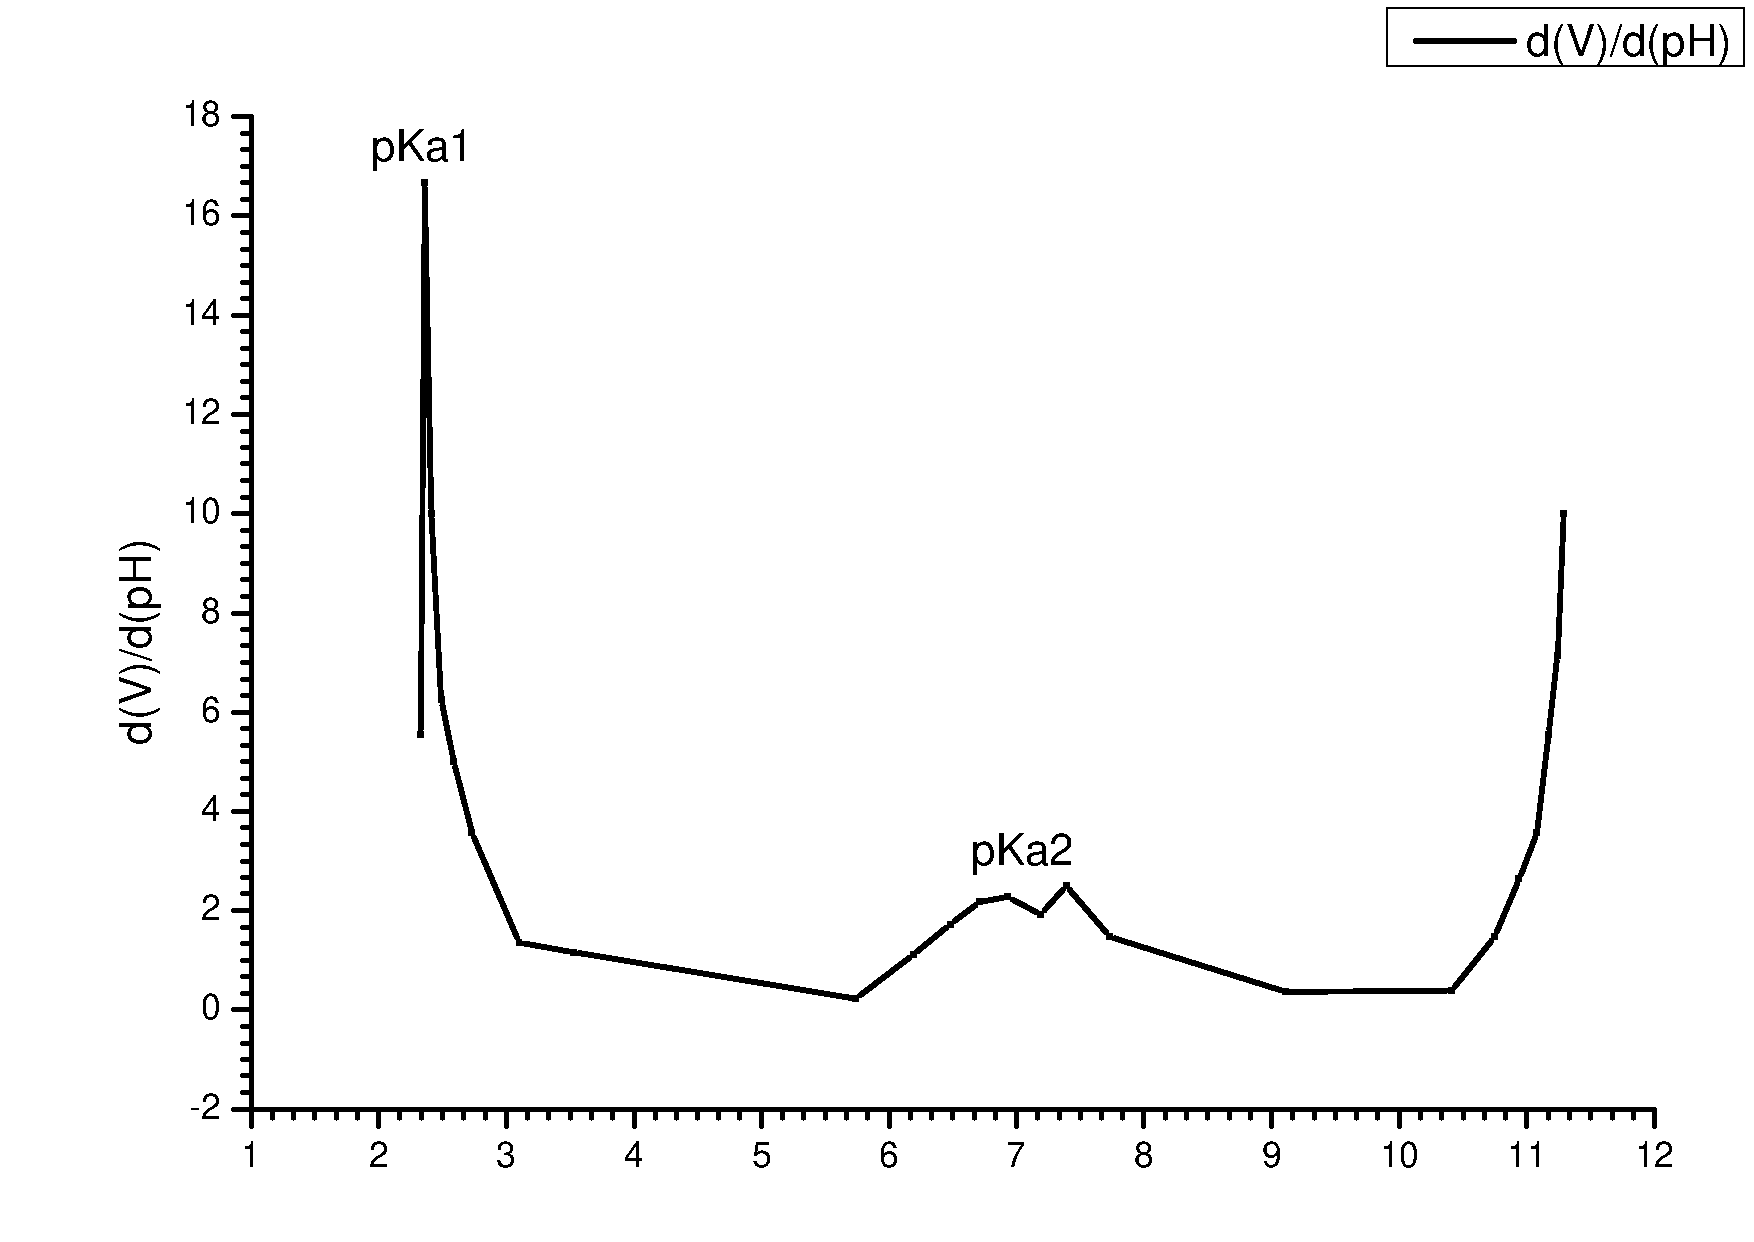
\includegraphics[scale=0.5]{integral.pdf}

\caption{Интегральная кривая титрования}

\label{fig:mpr}
\end{figure} 


\subsection{Теоретическая справка}
При титровании происходили следующие реакции:
\begin{equation}
\mathrm{H_3PO_4 + NaOH \rightleftarrows NaH_2PO_4 + H_2O}
\end{equation}
\begin{equation}
\mathrm{NaH_2PO_4 + NaOH \rightleftarrows Na_2HPO_4 + H_2O}
\end{equation}
\begin{equation}
\mathrm{Na_2HPO_4 + NaOH \rightleftarrows Na_3PO_4 + H_2O}
\end{equation}
На построенных кривых титрования отмечены основные точки содержащие в себе информацию об этом титровании и титруемой к-те. Так, точка эквивалентности соответствует полному образованию одной из солей и соотвтественно, моменту полной диссоциации форм к-ты, образующих эти соли. pH = $pK_{a}$, при котором молярные концентрации форм кислоты равны.При этом V составляет половину от $V_{т.экв}$.
\begin{gather}
\mathrm{HA \rightleftarrows H^+ + A^-} \quad K = \dfrac{[H^+][A^-]}{[HA]} \quad \Rightarrow \quad pH = pK_{a} + \lg \dfrac{[A^-]}{[HA]}
\end{gather}
\subsection{Анализ кривых}
\begin{enumerate}
\item По пикам дифференциальной кривой, определим точки эквивалентности. $T_{экв.1}$ наступила при $pH \approx 5.74$, $T_{экв.2}$ при $pH \approx 5.74$. До $T_{экв.3}$ не удалось дойти, но т.к. ортофосфорная к-та по 3 ступени крайне слабая в $T_{экв.3}$ скорее всего скачок бы отсутствовал.
\item По пикам интегральной кривой, определим $pK_{a}$. 
$pK_{a1}$ равно 2.33 pH, при табличном значении в 2.15, $pK_{a2}$ с некоторой погрешностью, равно 7,19 pH, при табличном значении в 7.20, $pK_{a3}$ сложнодостижима по нескольким причинам
\begin{itemize}
\item Титрование происходило только до pH = 11,29, поэтому на интегральной кривой нельзя рассмотреть зависимость, ведь по таблице $pK_{a3}$ = 12,35. 
\item $K_{a3}\approx K_{w}$, что означает, что $\mathrm{HPO_4^{2-}}$ очень плохо диссоциирует, поэтому эта точка была бы потеряна из-за статистических погрешностей.
\item Имела место протекающая бюретка и несовершенство pH метра.
\end{itemize}
\item Теоретическая концентрация была 0,01 М Точную концентрацию определим по формуле:
\begin{equation}
C_{H_3P0_4} = \dfrac{C_{NaOH}V_{NaOH}}{H_3P0_4}\approx0.009 М \quad \sigma=10%
\end{equation}
\end{enumerate}
\begin{figure}[H]

\centering

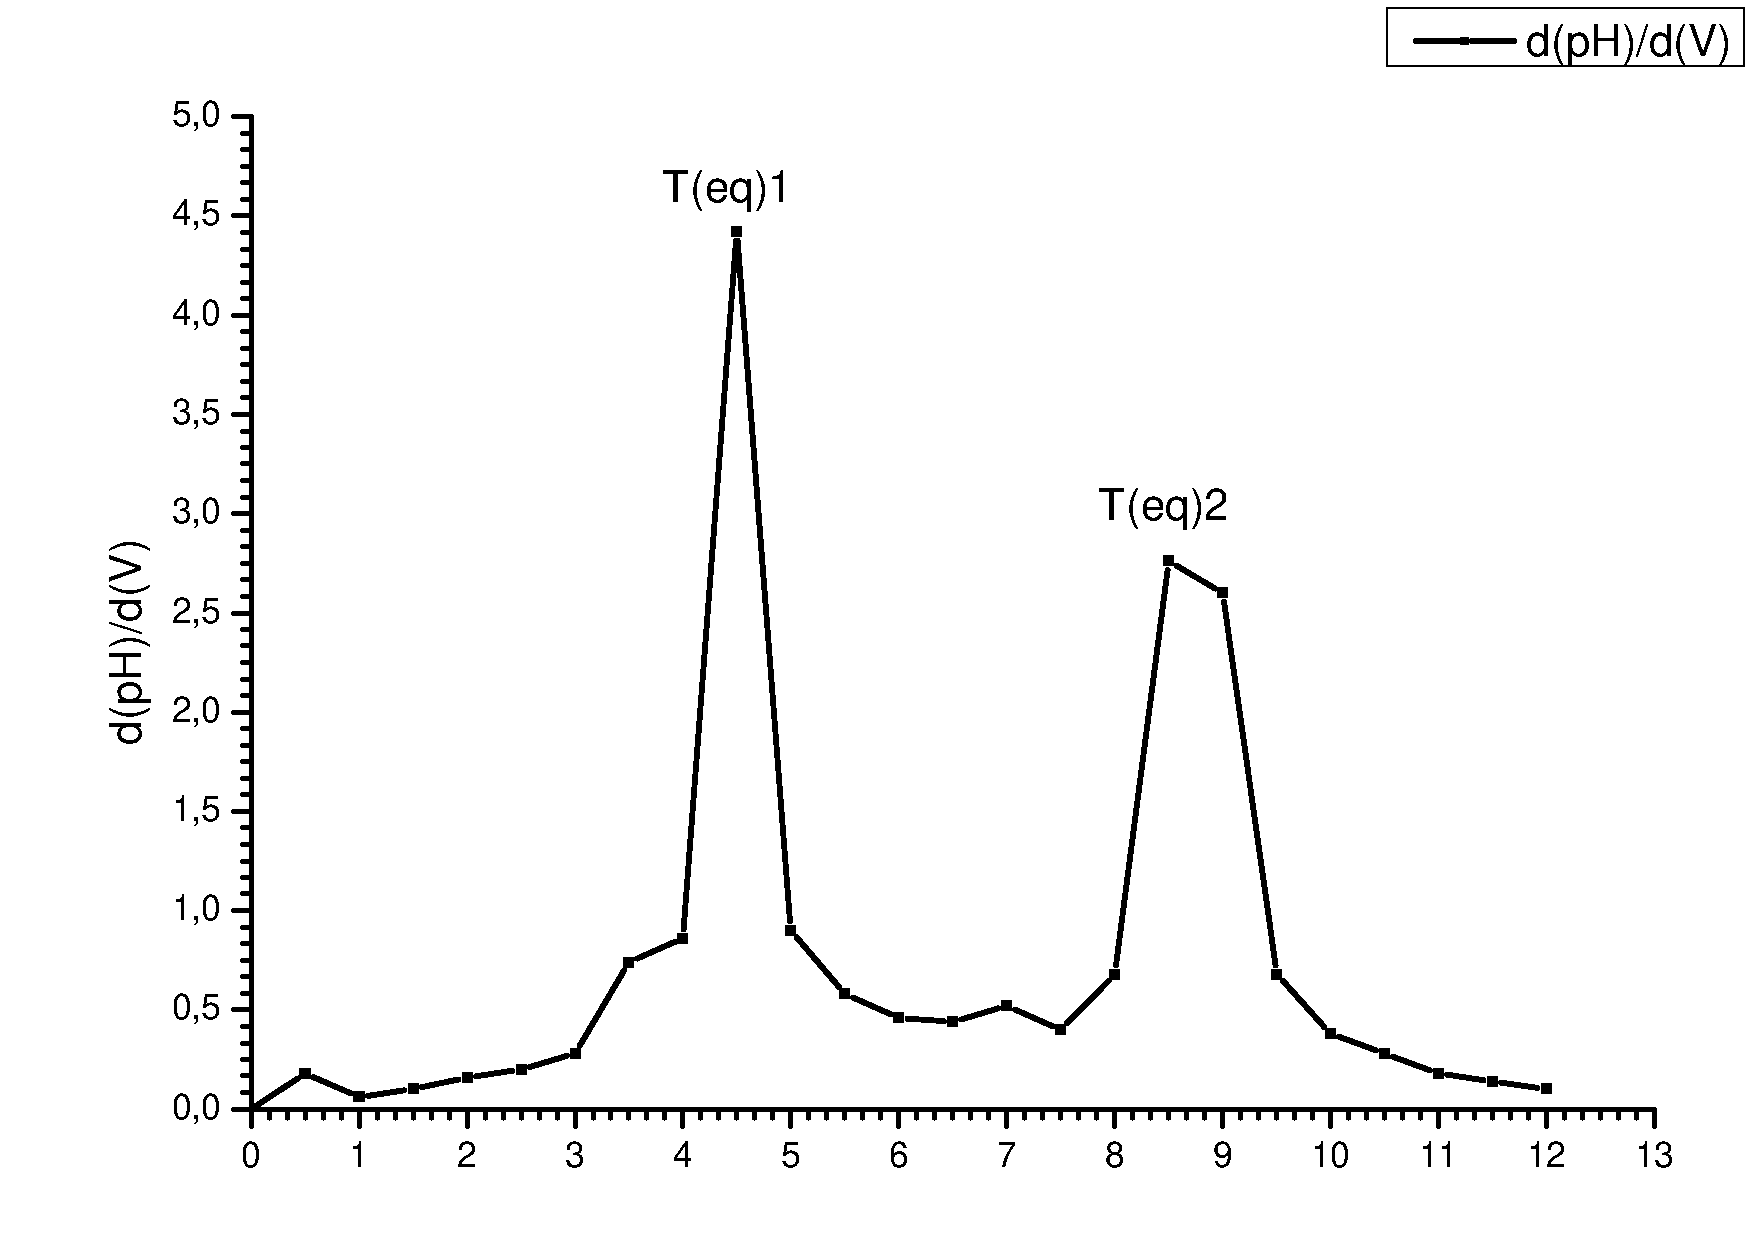
\includegraphics[scale=0.45]{diff.pdf}

\caption{Дифференциальная кривая титрования}

\label{fig:mpr}
\end{figure} 
\begin{figure}[H]

\centering

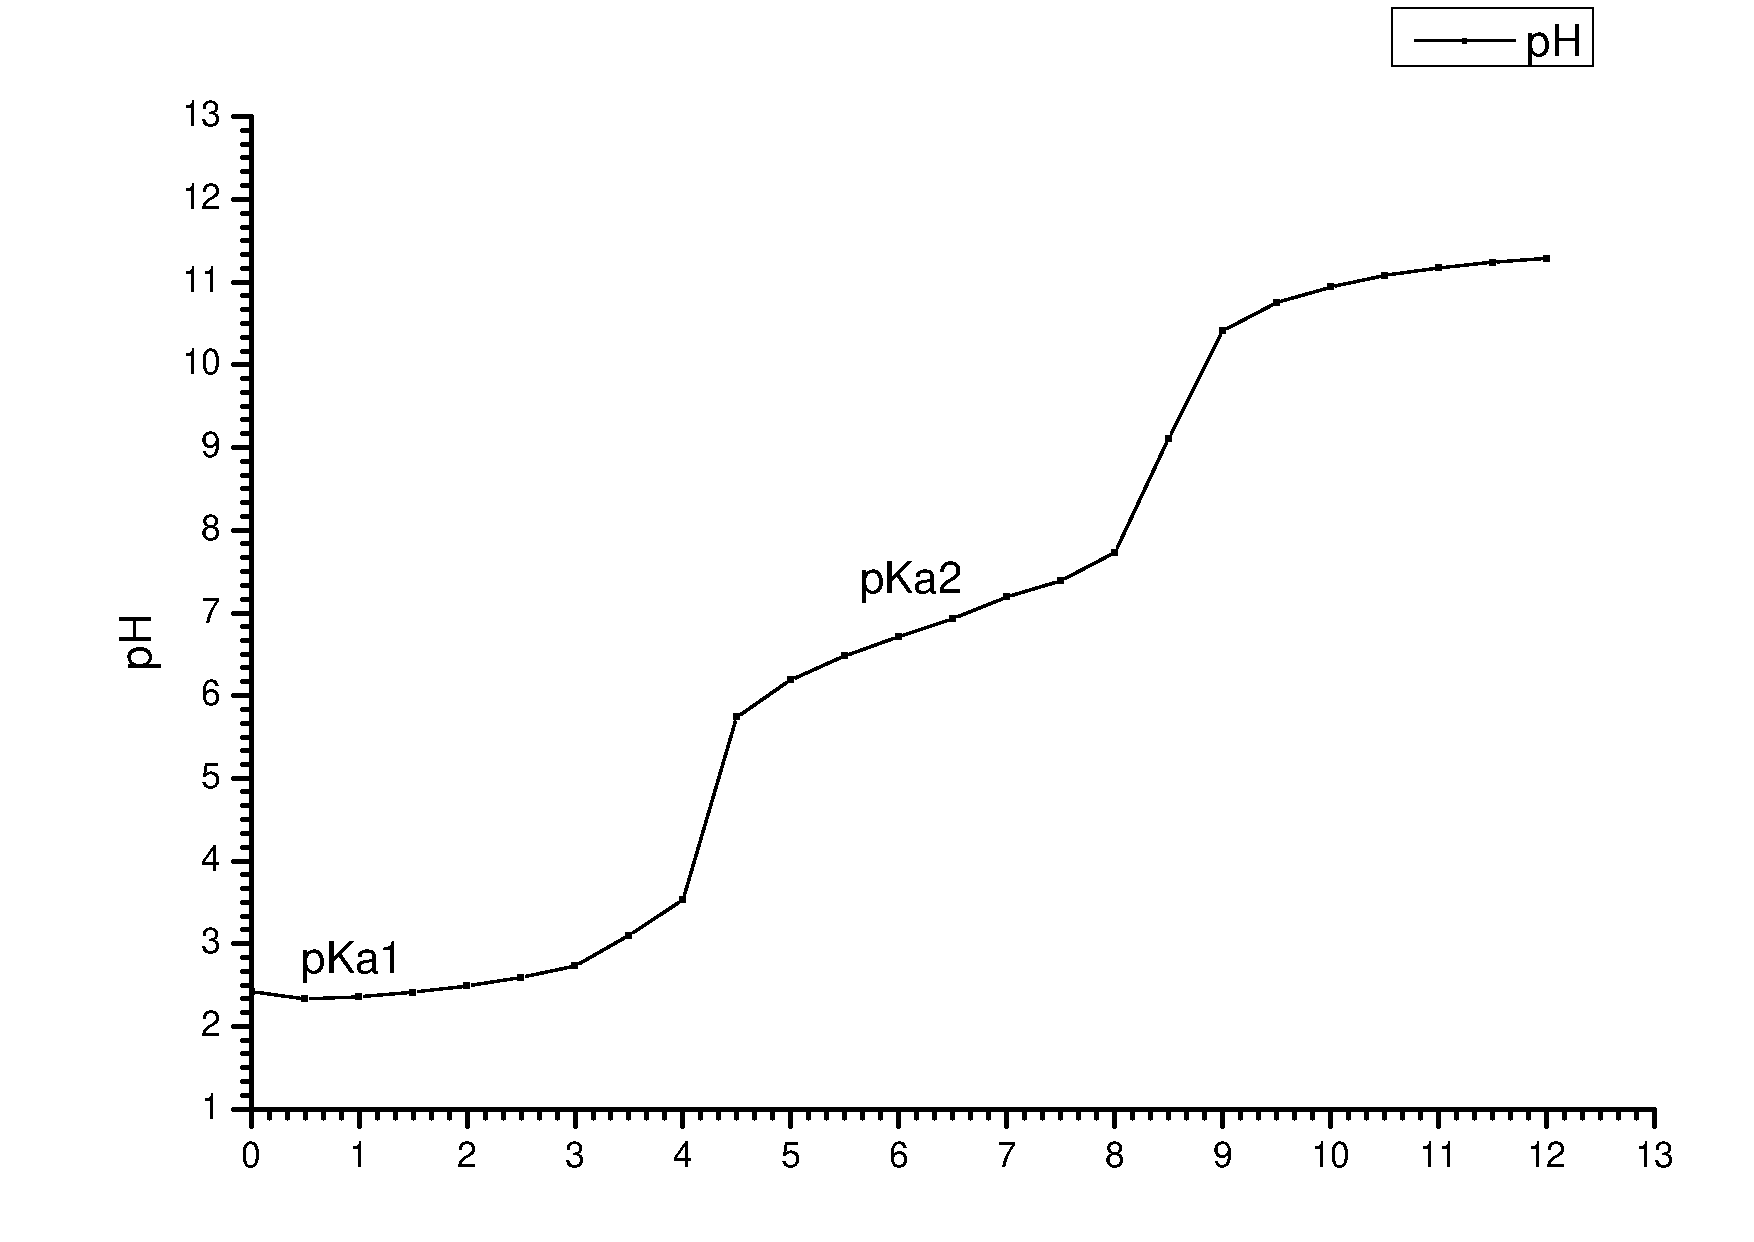
\includegraphics[scale=0.45]{common.pdf}

\caption{Обычная кривая титрования}

\label{fig:mpr}
\end{figure}
 Использованный индикатор - тимолфталеин, поменял окраску при pH между 9.11 и 10.41, а значит его можно использовать для приблизительного нахождения $T_{экв.2}$.
\section{Буферные растворы}
\subsection{Приготовление буферного раствора}
Взяли четыре пробирки. В первые две с помощью мерной пипетки налили по 1
мл 0,1М растворов дигидрофосфата натрия и гидрофосфата натрия в каждую.
Содержимое этих пробирок перемешали. Во вторые две пробирки внесли по 2 мл
дистиллированной воды. Во все пробирки добавили по 2 капли универсального
индикатора (или бромтимоловый синий).

Пробирки с дистиллятом приобрели желтоватый окрас, а пробирки с фосфатами - зеленоватый.
\subsection{Изучение свойств буферного раствора}
Добавили в 1ю и 3ю пробирки (буферный раствор и вода, соответственно) по
одной капле 0,1М раствора NaOH, следя за изменением цвета индикатора. 
После добавления \textbf{1 капли} 0.1M раствора NaOH раствор в 3 пробирке сразу приобрёл \textbf{синюю окраску}, при добавлении в 1 пробирку - более интенсивный оранжевый окрас. После добавления \textbf{30 капель} 1 раствор стал \textbf{синим}. 

Аналогичный опыт провели во 2й и 4й пробирках (буферный раствор и вода),
добавляя в них по капле 0,1М раствора HCl до момента появления красной окраски
раствора. После добавления 1 капли 0.1M раствора HСl 4-й раствор стал розовым, \textbf{24 капли} потребовалось, чтобы 2-й раствор стал \textbf{розовым}.

Буферные системы представляют собой смесь кислоты (донора протонов) и сопряженного с ней основания (акцептора протонов), то есть частиц, различающихся на $H^+$. В растворе устанавливаются равновесия:
\begin{equation}
\mathrm{H_2O \rightleftarrows H^+ + OH^-}
\end{equation}
\begin{equation}
\mathrm{HA \rightleftarrows H^+ + A^-}
\end{equation}
Каждое из этих равновесий характеризуется своей константой: первое — ионным произведением воды, второе — константой диссоциации кислоты.При добавлении в систему сильной кислоты, она протонирует основание, входящее в буферную смесь, а добавление сильного основания связывает протоны и смещает второе равновесие в сторону продуктов, при этом в итоге концентрация  в растворе $H^+$ меняется незначительно.
\section{Выводы}
В рамках работы мы познакомились с основными видами кислотно-основных равновесий, происходящих в растворах солей, кислот и оснований, а также научились новому методу исследования - потенциометрическому титрованию и узнали больше о буферных системах.

\end{document}
